\chapter{\uppercase{NCTM Case Study}}
The National Center for Therapeutic Medicine (NCTM) was used as a test bed for the original methodology. NCTM is a building located on the campus of Texas A\&M University, in College Station, Texas. 

The National Center for Therapeutics Manufacturing (NCTM) combines the educational and manufacturing focuses of the biopharmaceutical industry. The NCTM building is approximately 150,000 ft\textsuperscript{2} with nearly 50,000 ft\textsuperscript{2} of educational facilities that include wet labs, culture facilities, large lecture halls, and a mock current Good Manufacturing Practice (cGMP) training suite. Around 120,000 ft\textsuperscript{2} is on the first level and 30,000 ft\textsuperscript{2} is on the second level. 

The cGMP Suite contains modern biopharmaceutical manufacturing equipment that students can use to learn industry practices. The wet labs are equipped with chemical fume hoods and the necessary electronic equipment for following standard operating procedures used in the biopharmaceutical industry. The lecture halls seat up to 120 students and have large floor to ceiling windows. There is also an Apple Computer laboratory with 48 workstations on the second floor. 

On the academic side there are three dedicated outdoor air handling units that serve seven child air handling units. Two of the air handling units are constant speed and the others are variable air volume. OAHU 1-1 serves its own wet lab and also feeds into AHU 1-1 and AHU 1-2. OAHU 1-2 serves AHU 1-3 and 1-4 on the first floor. OAHU 2-1 serves three children air handlers on the second floor, AHU 2-1, 2-2, and 2-3. 

This document focuses on the academic side of the building since Utilities and Energy services with Texas A\&M University are only allowed to make immediate changes to the HVAC system on this side. In summary, the important parameters concerning NCTM are that it houses several biopharmaceutical labs, it has an academic side that can be immediately changed and a manufacturing side that cannot be immediately changed, and relies on dedicated outdoor air handling units to pretreat outdoor air. 

\begin{table}
\centering
\caption{Occupied/Unoccupied scheduling for the AHUs as described.}
\label{tab:OnOffSched}
\begin{tabular}{l c c c}
\toprule
Level 			& OAHU	 	& AHU \# 	& AHU Schedule 		 \\
\midrule
Floor 1 Area B	& OAHU 1-1  & N/A		& 24/7 	 \\
Floor 1 Area B 	& OAHU 1-1 	& AHU 1-1	& 24/7 	 \\
Floor 1 Area B 	& OAHU 1-1	& AHU 1-2	& 6am - 6pm, M-F 	 \\
Floor 1 Area A 	& OAHU 1-2 	& AHU 1-3	& 6am - 8pm, M-F	 \\
Floor 1 Area A 	& OAHU 1-2	& AHU 1-4	& 6am - 8pm, M-F 	 \\
Floor 2 		& OAHU 2-1	& AHU 2-1	& 6am - 10pm, M-F 	 \\
Floor 2 		& OAHU 2-1 	& AHU 2-2	& 6am - 10pm, M-F	 \\
Floor 2			& OAHU 2-1	& AHU 2-3	& 6am - 10pm, M-F 	 \\
\bottomrule
\end{tabular}
\end{table}

\begin{figure}
    \centering
\includegraphics[]{Plots/TempRiseVsFlow-AHU-2-14.pdf}
\caption{Temperature rise due to the mixing of plenum air at the terminal box for FPVAV-2-14. }
\end{figure}

\begin{table}
\caption{Fan schedule information for the dedicated outdoor air handlers.}
\label{tab:OAFanSched}
\centering
\begin{tabular}{l c c}
\toprule
OAHU & Design OA CFM & HP \\
\midrule
OAHU 1-1 & 12,800 & 20 \\
OAHU 1-2 & 4,500 & 5 \\
OAHU 2-1 & 2,200 & 2 \\
\bottomrule
\multicolumn{1}{r}{Total:} & 19,500 & 27 \\
\end{tabular}
\end{table}

\begin{table}
\centering
\caption{Fan schedule information for the AHUs.}
\label{tab:FanSched}
\begin{tabular}{l c c c c}
\toprule
AHU 	& Type	 	& Total Airflow (CFM) 	& HP 	& OA Served By\\
\midrule
AHU 1-1 & Constant  & 3,000 			  	& 5 	& OAHU 1-1 \\
AHU 1-2 & VAV 		& 4,800 				& 5 	& OAHU 1-1 \\
AHU 1-3 & VAV 		& 7,500 				& 7.5 	& OAHU 1-2 \\
AHU 1-4 & Constant 	& 5,000 				& 7.5 	& OAHU 1-2 \\
AHU 2-1 & VAV 		& 6,000 				& 7.5 	& OAHU 2-1 \\
AHU 2-2 & VAV		& 8.500					& 10 	& OAHU 2-1 \\
AHU 2-3 & VAV 		& 6,000					& 7.5	& OAHU 2-1 \\
\bottomrule
\multicolumn{2}{r}{Total:} & 40,800 & 50 &  \\
\end{tabular}
\end{table}

\section{Terminal Unit Information}

On the academic side, there are a total of 10 series fan powered terminal units on the first floor and 18 on the second floor. Table \ref{tab:TerminalUnitInformation} shows the design (and assumed constant) flowrates for each of the terminal units. 

% Please add the following required packages to your document preamble:
% \usepackage{booktabs}
\begin{table}[]
\centering
\footnotesize
\caption{Terminal unit information.}
\label{tab:TerminalUnitInformation}
\begin{tabular}{@{}llrl@{}}
\toprule
AHU &  Terminal Unit & \parbox{1.5cm}{Flow\\(CFM) }& Space Served \\ \midrule
%%\parbox{2cm}{AHU-1-1 \\ (5 hp)} & \multicolumn{3}{l}{No boxes - Serves Teaching Module alone, Constant Fan} \\ \midrule
AHU-1-2        & FPVAV-1-7 & 1,400 & Difficult to tell \\ \cmidrule(r){2-4}
(5 hp)         & FPVAV-1-8 & 700 & Vestible/Men's \& Women's bathroom \\  \cmidrule(r){2-4}
               & FPVAV-1-9 & 1,200 & Stairs/Front Corridor \\  \cmidrule(r){2-4}
               & FPVAV-1-10 & 1,600 & Hallway \\\midrule
AHU-1-3        & FPVAV-1-1 & 1,480 & Large Auditorium Lecture Hall \\  \cmidrule(r){2-4}
(7.5 hp)       & FPVAV-1-2 & 1,160 & Large Auditorium Lecture Hall \\  \cmidrule(r){2-4}
               & FPVAV-1-3 & 1,300 & Large Auditorium Lecture Hall \\  \cmidrule(r){2-4}
               & FPVAV-1-4 & 1,400 & Large Auditorium Lecture Hall \\  \cmidrule(r){2-4}
               & FPVAV-1-5 & 1,040 & Large Auditorium Lecture Hall \\  \cmidrule(r){2-4}
               & FPVAV-1-6 & 1,120 & Large Auditorium Lecture Hall \\\midrule
%%\parbox{2cm}{AHU-1-4 \\ (7.5 hp)} & \multicolumn{3}{l}{No boxes - Serves open atrium outside lecture halls, constant fan}  \\\midrule
AHU-2-1  & FPVAV-2-1 & 2,000 & Large Study Area \\  \cmidrule(r){2-4}
        (7.5 hp)   & FPVAV-2-2 & 2,200 & Large Study Area \\  \cmidrule(r){2-4}
               & FPVAV-2-3 & 1,800 & Open Corridor \\\midrule
AHU-2-2  & FPVAV-2-9 & 2,400 & Computer Lab \\  \cmidrule(r){2-4}
         (10 hp)      & FPVAV-2-12 & 500 & Kitchen/Mail Room \\  \cmidrule(r){2-4}
               & FPVAV-2-13 & 1,000 & Open Corridor \\  \cmidrule(r){2-4}
               & FPVAV-2-14 & 850 & \pbox{\textwidth}{Men's/Women's Restroom \\ Copy/Mail \\ Waiting Area }\\  \cmidrule(r){2-4}
               & FPVAV-2-15 & 1,400 & Reception/Seating/Admin Lobby \\  \cmidrule(r){2-4}
               & FPVAV-2-16 & 500 & Small Conference Room \\  \cmidrule(r){2-4}
               & FPVAV-2-17 & 1,280 & 4 Small Offices \\  \cmidrule(r){2-4}
               & FPVAV-2-18 & 600 & Large Office \\\midrule
AHU-2-3  & FPVAV-2-4 & 2,000 & Open Corridor \\  \cmidrule(r){2-4}
        (7.5 hp)       & FPVAV-2-5 & 600 & Open Seating \\  \cmidrule(r){2-4}
               & FPVAV-2-6 & 400 & Small Conference Room \\  \cmidrule(r){2-4}
               & FPVAV-2-7 & 200 & Office \\  \cmidrule(r){2-4}
               & FPVAV-2-8 & 1,200 & Visitor Conference \\  \cmidrule(r){2-4}
               & FPVAV-2-10 & 540 & 3 Sponsor Offices \\  \cmidrule(r){2-4}
               & FPVAV-2-11 & 560 & 3 Sponsor Offices \\ \bottomrule
\end{tabular}
\end{table}


\section{Analysis of Zone Load Predictions}

An important factor in the optimization methodology is the prediction of the zone loads at a given time, without access to current live sensor information. 

Before analyzing the prediction ability of different zone loads, it is important to gather insight into the nature of the calculated variable that is proposed to be used as the surrogate for zone load.   

If the zone loads are being met and steady-state conditions are assumed, the sensible zone load will be

\begin{equation}
    Q_{zone}=\flow{z} \rhocp{} \left(T_{dis}-T_{z} \right) \approx 1.1 \cdot \flow{z}\left(T_{dis}-T_{z} \right)
\end{equation}

A useful simplification would be replacing the \(\rhocp{}\) term with a constant value. A value of 1.1, when \(\flow{z}\) is in units of CFM and temperature is in units of \(^\circ\)F is common. 

Figure \ref{fig:ZoneLoadforContainerFPVAV214vsOADryBulbTemperatureNOAA} shows an example of the zone load plotted against outdoor air dry-bulb temperature. Notice that the load is not a well defined function of outdoor air temperature. This turns out to be the case for many of the internal zones, which will be related more to the time of day parameters. 

Figure \ref{fig:ZoneLoadForContainer29vsNOAAOAT} shows the zone load for FPVAV-2-9 versus outdoor air Temperature. FPVAV-2-9 serves only internal zones, and the load only ranges from approximately 250 BTU/hr to 4,000 BTU/hr. 




\begin{figure}
\centering
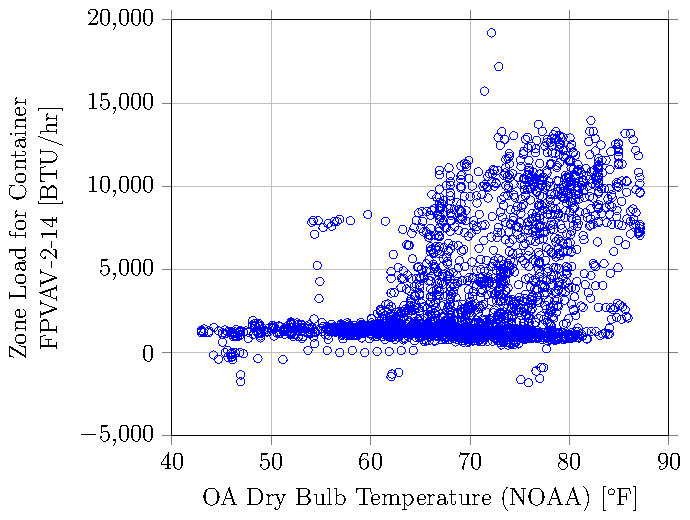
\includegraphics{Plots/CalculatedZoneLoadFPVAV-2-14.pdf}
\caption{Calculated zone load for FPVAV-2-14 during the month of April 2016.}
\label{fig:ZoneLoadforContainerFPVAV214vsOADryBulbTemperatureNOAA}
\end{figure}


\begin{figure}
\centering
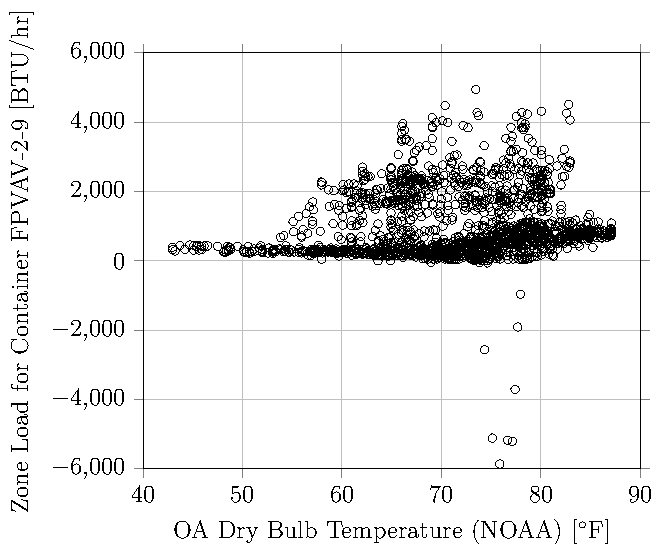
\includegraphics{Plots/CalculatedZoneLoad-2-9.pdf} 
\caption{Calculated zone load for FPVAV-2-9, which serves only internal space, during the month of April 2016.}
\label{fig:ZoneLoadForContainer29vsNOAAOAT}
\end{figure}


\section{Analysis of the Mixed Air Temperature and Reheat Assumption}

For series fan powered boxes, the assumption was made that the total flow remains constant and that the mixed air temperature at the individual box can be predicted based on the primary flow value that is measured. 


\section{Analysis of the Critical Zone Assumption}

The critical zone/damper is to be used to determine the static pressure setpoint that can be used to supply the desired flows found from the optimization. An important consideration in the methodology is checking how how this assumption holds. Data from NCTM can be used to test the validity of the approach.


The following figures show the maximum damper position of the children terminal units for each of the air handlers during the month of April 2016. During this time, for AHU-2-1 and AHU-2-2, there was no time in which a terminal unit damper was fully open which indicates that there is potential for the supply air static pressure setpoint to be reduced.  

\begin{figure}
\centering
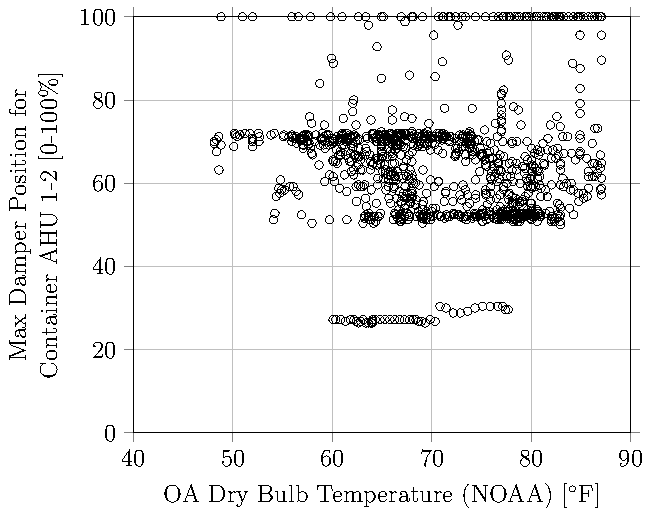
\includegraphics{Plots/MaximumDamperPosition-1-2.pdf} 
\caption{Maximum damper position versus outside air temperature for AHU-1-2 during the month of April 2016.}
\label{fig:MaxDamperPositionforContainerAHU12vsOADryBulbTemperatureNOAA}
\end{figure}

\begin{figure}
\centering
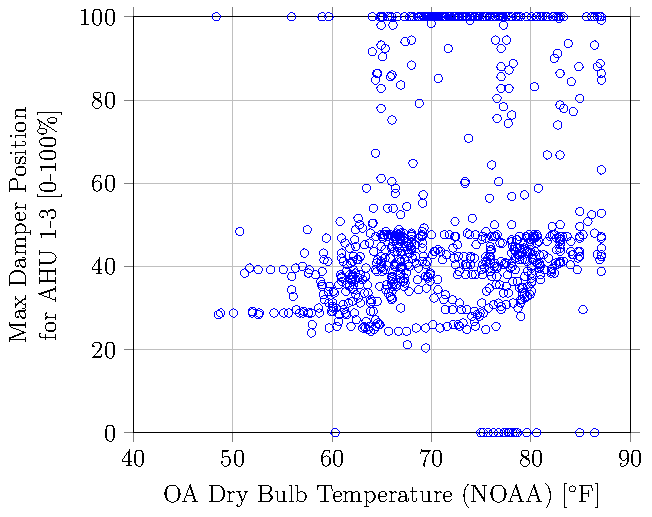
\includegraphics{Plots/MaximumDamperPosition-1-3.pdf}
\caption{Maximum damper position versus outside air temperature for AHU-1-3 during the month of April 2016.}
\label{fig:MaxDamperPositionforContainerAHU13vsOADryBulbTemperatureNOAA}
\end{figure}


\begin{figure}
\centering
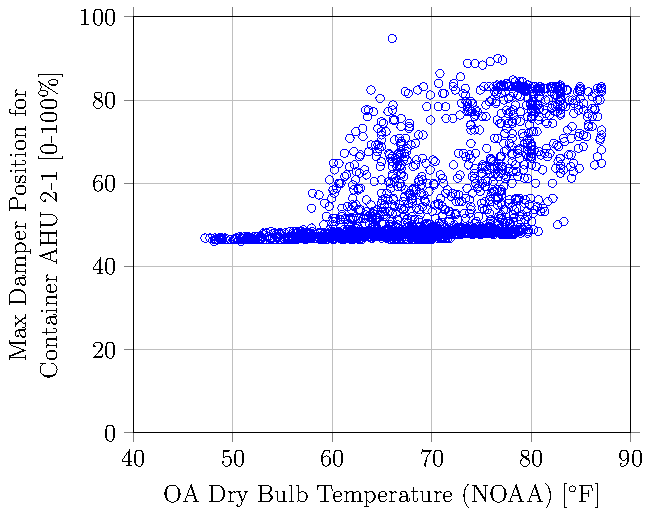
\includegraphics{Plots/MaximumDamperPosition-2-1.pdf}
\caption{Maximum damper position versus outside air temperature for AHU-2-1 during the month of April 2016.}
\label{fig:MaxDamperPositionforContainerAHU21vsOADryBulbTemperatureNOAA}
\end{figure}

